\PassOptionsToPackage{dvipsnames}{xcolor}
\documentclass[hyperref,UTF8,notheorems,xcolor={dvipsnames}]{beamer}
\usepackage[dvipsnames]{xcolor}
\usetheme{Rochester}
\usepackage{amsmath, mathtools, graphicx}
\usepackage{standalone}
\usepackage[most]{tcolorbox}
\usepackage[normalem]{ulem}
\usepackage{xeCJK}
\usepackage{fontspec}

\usepackage{tikz}
\usetikzlibrary{positioning,arrows.meta,bending}

\usepackage{pgfplots}
\usepackage{pifont}
\usepackage{fontawesome5}
\usepgfplotslibrary{polar}
\usepgflibrary{shapes.geometric}
\usetikzlibrary{calc,angles,quotes}
\defaultfontfeatures{Mapping=tex-text}
\usefonttheme{professionalfonts}
\usepackage{concmath}
\usepackage{minted}

\newcommand{\cmark}{\ding{51}}%
\newcommand{\xmark}{\ding{55}}%

\newcommand{\CC}[1]{#1}

\newcommand{\Cincluded}{{\small\cmark}}
\newcommand{\Cdefine}{{\small\cmark\faFile*[regular]}}
\newcommand{\Ccodeonly}{{\small\cmark\faFile*~}}
\newcommand{\Cnofocus}{{\small\faQuestion}}
\newcommand{\Cexmaybe}{{\small\xmark\faQuestionCircle}}
\newcommand{\Cexcluded}{{\small\xmark}}

\newcommand{\Iincluded}{\item[\hbox to 1.8em{\Cincluded\hfill}]}
\newcommand{\Idefine}{\item[\hbox to 1.8em{\Cdefine\hfill}]}
\newcommand{\Icodeonly}{\item[\hbox to 1.8em{\Ccodeonly\hfill}]}
\newcommand{\Inofocus}{\item[\hbox to 1.8em{\Cnofocus\hfill}]}
\newcommand{\Iexmaybe}{\item[\hbox to 1.8em{\Cexmaybe\hfill}]}
\newcommand{\Iexcluded}{\item[\hbox to 1.8em{\Cexcluded\hfill}]}

\DeclareRobustCommand{\rddots}{\text{\reflectbox{$\ddots$}}}


\usepackage{graphicx}
\graphicspath{ {./../images/} }

\def\codesize{\fontsize{8}{9}\selectfont}
\setmonofont[Mapping=]{Source Code Pro}
\setminted{fontsize=\codesize, linenos, frame=lines, mathescape, autogobble, tabsize=4}
\setCJKmainfont[AutoFakeSlant,BoldFont=Noto Sans CJK TC Bold]{Noto Sans CJK TC}

\setlength{\parskip}{\baselineskip} 
\newcommand{\btitle}[1]{{\secname} -- #1}
\newcommand{\stitle}[1]{{\subsecname} -- #1}

\theoremstyle{definition}
\newtheorem{theorem}{定理}
\newtheorem{lemma}{引理}
\newtheorem{property}{性質}
\newtheorem{corollary}{推論}
\newtheorem{problem}{例題}


\newtheorem{definition}{定義}
\AtBeginEnvironment{definition}{
  \setbeamercolor{block title}{fg=white,bg=red!70!black}
  \setbeamercolor{block body}{fg=black, bg=block title.bg!10!bg}
}

\newtheorem{exercise}{習題}
\AtBeginEnvironment{exercise}{
  \setbeamercolor{block title}{fg=white,bg=green!30!black}
  \setbeamercolor{block body}{fg=black, bg=block title.bg!10!bg}
}


\AtBeginSection[]{
%   \begin{frame}
%     \tableofcontents[currentsection,hideallsubsections]
%   \end{frame}
  \begin{frame}
  \vfill
  \centering
  \begin{beamercolorbox}[sep=6pt,center,shadow=true,rounded=true]{title}
    \usebeamerfont{title}\LARGE\insertsectionhead\par%
  \end{beamercolorbox}
  \vfill
  \end{frame}
}

\AtBeginSubsection[]{
  \begin{frame}[shrink]{\btitle{\subsecname}}
    \setlength{\parskip}{8pt}
    \tableofcontents[subsectionstyle=show/shaded/hide, sectionstyle=show/hide, subsubsectionstyle=hide/hide/hide/hide]
  \end{frame}
}

\AtBeginSubsubsection[]{
  \begin{frame}[shrink]{\stitle{\subsubsecname}}
    \setlength{\parskip}{8pt}
    \tableofcontents[subsectionstyle=show/hide/hide, sectionstyle=show/hide, subsubsectionstyle=show/shaded/hide/hide]
  \end{frame}
}

\usepackage{ctable}
\usepackage{tabularx}

\setlength{\parskip}{\baselineskip}

\usepackage{listings}

\lstset{language=C++,
                basicstyle=\ttfamily\small,
                breaklines=true,
                numbers=left,
                numberstyle=\tiny,
                frame=single,
                keywordstyle=\color{blue}\ttfamily,
                stringstyle=\color{red}\ttfamily,
                commentstyle=\color{gray}\ttfamily,
                morecomment=[l][\color{magenta}]{\#}
}

\title{Data Sctructure}

\hypersetup{CJKbookmarks=true}
\begin{document}

\author{謝嘉穎}
\date{TODO TODO 2025}

\frame{\titlepage}

\begin{frame}[fragile]{講師介紹}
  \begin{itemize}
    \item 謝嘉穎
    \pause
    \item BLAME (blameazu)
    \pause
    \item 因為想學資料結構,所以來當資料結構講師
  \end{itemize}
\end{frame}

\begin{frame}[fragile]{前言}
  今天這堂課是教資料結構,雖然課堂上只會講概念,並不會有時間給大家實作。
  \pause

  但希望大家可以先把概念記下來,閒暇時間再自行練習實作。
  \pause

  然後講師應該塞了很多東西進來,\sout{聽到後面聽不懂應該是正常的}
  \pause

  假如大家覺得太簡單/難,可以自己去練題目
  \pause

  但盡量跟上課內容是更好的! omob
\end{frame}

\begin{frame}[fragile]{上課大綱}
  \tableofcontents[sectionstyle=show/show, hideallsubsections,sections={1-3}]
\end{frame}

\section{基礎資料結構}

\begin{frame}[fragile]{\btitle{大綱}}
  \setlength{\parskip}{8pt}
  \tableofcontents[subsectionstyle=show/show/hide, sectionstyle=show/hide, subsubsectionstyle=hide/hide/hide/hide]
\end{frame}

\subsection{資料結構介紹}

\begin{frame}[fragile]{\stitle{前言}}
  什麼是資料結構?
  \pause

  在電腦科學中,資料結構(英語:data structure)是電腦中儲存、組織資料的方式。 by wiki
  \pause

  能將資料結構當成一個工具盒
  \pause

  在特殊的情況下找到對應的工具盒是非常重要的
\end{frame}

\begin{frame}[fragile]{\stitle{Example}}
  \begin{problem}
    有一個隊伍

    $Q$ 筆操作,共有 $2$ 種操作
    \begin{enumerate}
      \item 每次從隊伍後端加入編號為 $A_i$ 的人
      \item 每次從隊伍前端拔除一個人,並且需要輸出最前端的人是誰
    \end{enumerate}
  \end{problem}
  \pause

  假如你有認真上 STL 課的話
  \pause
  queue!
  \pause

\begin{lstlisting}
queue<int> qq;
qq.push(a); // add
qq.pop(); // remove
\end{lstlisting}
  \pause

  而 \lstinline|push| 及 \lstinline|pop| 就是我們與這個工具盒的互動
\end{frame}

\begin{frame}[fragile]{\stitle{總結}}
  也就是說一個能儲存資料、整理資料、拿取資料的工具包

  我們其實就可以簡單的稱為 \textbf{資料結構}
  \pause

  而資料結構之間有些並無好壞之分
  \pause

  像是要用到 First In First Out 的題目,你用 queue 解

  Last in First Out 的題目,你用 stack 解
  \pause

  針對這些性質上的差異,我們選取一個 \textbf{"適當"} 的資料結構
\end{frame}

\subsection{Struct \& Class}

\subsubsection{Struct 介紹}

\begin{frame}[fragile]{\stitle{\subsubsecname}}
  Struct 是 C++ 中的一個語法

  中文應該叫做結構(Structure)
  \pause

  是一種把一大堆變數、資料丟在一起

  使得方便管理他們的地方
\end{frame}

\begin{frame}[fragile]{\stitle{\subsubsecname}}
  也可以想像 Struct 是一個紙皮箱
  \pause

  你可以把很多個物品丟進去裡面,最後用膠帶封起來
  \pause

  而你又可以想像,那個紙皮箱上有兩個小孔,分別是 Input 跟 Output
  \pause

  所以你唯一溝通整個紙箱子的通道就只有那兩個孔,可以丟東西進去 or 取東西出來
  \pause

  \sout{當然不排除有把箱子拆開把東西直接拿出來的功能}
\end{frame}

\begin{frame}[fragile]{\stitle{\subsubsecname}}
  蛤? 跟把變數宣告在外面有什麼差別?
  \pause

  你可以想像箱子裡有一個自動運轉的機器
  \pause

  當你把東西 Ex. 統一布丁、奶茶 丟進去,機器會自動將物品按照某種特定的方式整理好
  \pause

  所以當你在箱子外面要把東西取出來的時候,會很方便 (畢竟都幫你整理好了)
\end{frame}

\begin{frame}[fragile]{\stitle{\subsubsecname}}
  舉例來講,有一個Struct 他在內部會將資料做 Merge Sort 的整理。
  \pause

  \includegraphics[width=\textwidth]{./photos/struct_ex.png}
\end{frame}

\subsubsection{Struct 語法}

\begin{frame}[fragile]{\stitle{\subsubsecname}}
\begin{lstlisting}
struct name {
  // 變數
  int b = 0;
  name(/*可以放參數在這裡面*/) {
    // 初始化東西可以放這裡
  }
  // 底下可以寫 function
  void f() {
    cout << "Hello_World!\n";
  }
};
\end{lstlisting}
\end{frame}

\begin{frame}[fragile]{\stitle{\subsubsecname}}
  \begin{lstlisting}
    name a(/*可以放參數在這裡面*/);
    // a 是變數名稱
    a.f(/*參數*/); // 呼叫 f function
    a.b += 2; // 可以進去修改參數 or 拿出來
  \end{lstlisting}
\end{frame}

\subsubsection{Class 介紹}

\begin{frame}[fragile]{\stitle{\subsubsecname}}
  Class
  \pause

  我也不會,沒用到過。
\end{frame}

\subsection{並查集 (Disjoint Set Union)}

\begin{frame}[fragile]{\stitle{大綱}}
  \setlength{\parskip}{8pt}
  \tableofcontents[subsectionstyle=show/hide/hide, sectionstyle=show/hide, subsubsectionstyle=show/show/hide/hide]
\end{frame}

\subsubsection{一些基礎圖論的東西}

\begin{frame}[fragile]{\stitle{\subsubsecname}}
  什麼是 圖論(Graph)
  \pause

  圖論在 Computer Science 中是一門重要的主題
  \pause

  圖論所主要研究的主題是圖
  \pause

  圖是由若干個節點,以及連接相鄰兩點的邊所構成的圖形。
\end{frame}

\begin{frame}[fragile]{\stitle{\subsubsecname}}
  節點 (Nodes, Vertexs)
  \pause

  這張圖就是有三個節點,$A$、$B$、$C$
  
  \centering
  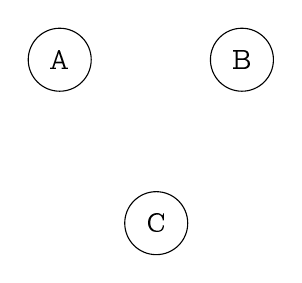
\begin{tikzpicture}[every node/.style={circle, draw, minimum size=8mm}]
    \node (A) {A};
    \node (B)[right=1.5cm of A] {B};
    \node (C)[below right=1.5cm and 0.65cm of A] {C};
  \end{tikzpicture}
\end{frame}

\begin{frame}[fragile]{\stitle{\subsubsecname}}
  邊 (Edges)
  \pause

  這張圖就是有三個節點,$A$、$B$、$C$
  
  三條邊 $A \to B$、$B \to C$、$C \to A$
  
  \centering
  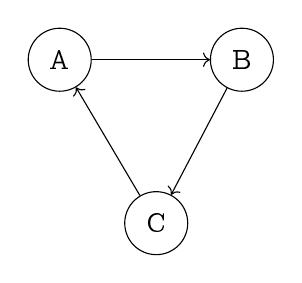
\begin{tikzpicture}[every node/.style={circle, draw, minimum size=8mm}]
    \node (A) {A};
    \node (B)[right=1.5cm of A] {B};
    \node (C)[below right=1.5cm and 0.65cm of A] {C};
    \draw[->] (A) -- (B);
    \draw[->] (B) -- (C);
    \draw[->] (C) -- (A);
  \end{tikzpicture}
  \pause
  \centering
  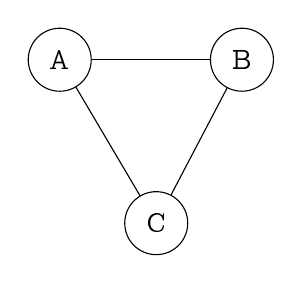
\begin{tikzpicture}[every node/.style={circle, draw, minimum size=8mm}]
    \node (A) {A};
    \node (B)[right=1.5cm of A] {B};
    \node (C)[below right=1.5cm and 0.65cm of A] {C};
    \draw (A) -- (B);
    \draw (B) -- (C);
    \draw (C) -- (A);
  \end{tikzpicture}

  左邊跟右邊這張圖是有向邊與無向邊的差異
\end{frame}

\begin{frame}[fragile]{\stitle{\subsubsecname}}
  連通塊 (Connected Component)
  \pause

  當二節點 $A$、$B$,且 $A$ 節點與 $B$ 節點可以透過邊互相到達(不管邊的方向),則 $A$、$B$ 視為在同一個連通塊當中
  \pause
  
  \centering
  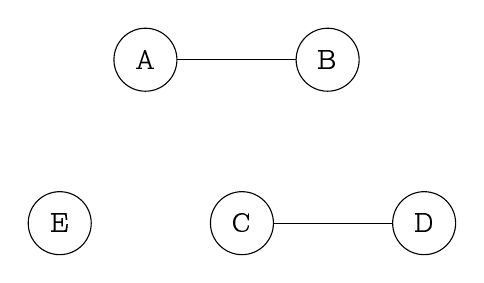
\begin{tikzpicture}[every node/.style={circle, draw, minimum size=8mm}]
    \node (A) {A};
    \node (B)[right=1.5cm of A] {B};
    \node (C)[below right=1.5cm and 0.65cm of A] {C};
    \node (D)[right=1.5cm of C] {D};
    \node (E)[left=1.5cm of C] {E};
    \draw (A) -- (B);
    \draw (C) -- (D);
  \end{tikzpicture}

  $\{A, B\}$ 為一連通塊,$\{C, D\}$ 為一連通塊,$\{E\}$ 為一連通塊
\end{frame}

\subsubsection{DSU 介紹}

\begin{frame}[fragile]{\stitle{\subsubsecname}}
  Disjoint Set Union (並查集)
  \pause
  ,通常我們都簡稱 DSU
  \pause

  是一種用來解決圖論上節點連通狀塊的資料結構
  \pause
  
  雖然通常都是拿來合併集合之類的,但大部分都可以抽象化為圖論去思考
  \pause

  DSU 支援的操作
  \pause
  \begin{itemize}
    \item 將兩個節點相連
    \pause
    \item 詢問兩點的連通關係
  \end{itemize}
\end{frame}

\begin{frame}[fragile]{\stitle{\subsubsecname}}
  我們先定義在 DSU 中,所有的節點都有他們的唯一出邊,一開始所有節點的出邊都是指向自己
  \pause

  \begin{tikzpicture}[every node/.style={circle, draw, minimum size=8mm},
                      every loop/.style={looseness=10, min distance=5mm}]
    \node (A) {A};
    \node (B)[right=1.5cm of A] {B};
    \node (C)[below right=1.5cm and 0.65cm of A] {C};
    \draw[->] (A) edge[loop above] (A);
    \draw[->] (B) edge[loop right] (B);
    \draw[->] (C) edge[loop below] (C);
  \end{tikzpicture}
\end{frame}

\begin{frame}[fragile]{\stitle{\subsubsecname}}
  假設我們今天的圖的每個連通塊都有一個性質
  \pause

  每個連通塊皆具有一個唯一的結束點,也就是說不管從哪個節點開始順著邊走,我們最後都將會走到同一節點上,且那個節點的邊指向自己
  \pause

  \begin{columns}
    \begin{column}{0.5\textwidth}
      \centering
      \begin{tikzpicture}[every node/.style={circle, draw, minimum size=8mm},
                      every loop/.style={looseness=10, min distance=5mm}]
        \node (A) {A};
        \node (B)[below left=1cm and 0.65cm of A] {B};
        \node (C)[below right=1cm and 0.65cm of A] {C};
        \node (D)[below right=1cm and 0.65cm of C] {D};
        \draw[->] (A) edge[loop above] (A);
        \draw[->] (B) -- (A);
        \draw[->] (C) -- (A);
        \draw[->] (D) -- (C);
      \end{tikzpicture}
    \end{column}
    \pause
    \begin{column}{0.5\textwidth}
      \centering
      每個點最終都會匯集到點 $A$
      \begin{itemize}
        \item $A$
        \pause
        \item $B \to A$
        \pause
        \item $C \to A$
        \pause
        \item $D \to C \to A$
      \end{itemize}
      \pause

      那麼當我們詢問兩點是否在同一個連通塊,就等價於問他們的結束點是否相同
    \end{column}
  \end{columns}
\end{frame}

\begin{frame}[fragile]{\stitle{\subsubsecname}}
  那麼我們在連接點 $A$、點 $B$ 時,我們就必須要確保這個性質一直都會存在!
  \pause

  那麼我們可以發現,連通塊 $A$ 與連通塊 $B$ 皆具有自己的一個結束點
  \pause

  但當我們將他們合併成一個大連通塊 $C$,$C$ 只能具有一個結束點而已
  \pause

  所以我們就將 $A$ 的結束點連接到 $B$ 的結束點即可!
\end{frame}

\begin{frame}[fragile]{\stitle{\subsubsecname}}
  \centering
  合併連通塊 $A$ 與 連通塊 $B$

  \begin{tikzpicture}[every node/.style={circle, draw, minimum size=8mm},
                  every loop/.style={looseness=10, min distance=5mm}]
    \node (A) {A};
    \node (B)[below left=1cm and 0.65cm of A] {B};
    \node (C)[below right=1cm and 0.65cm of A] {C};
    \node (D)[below right=1cm and 0.65cm of C] {D};
    \node (E)[right=3cm of A] {E};
    \node (F)[below right=1cm and 0.65cm of E] {F};
    \draw[->] (A) edge[loop above] (A);
    \draw[->] (B) -- (A);
    \draw[->] (C) -- (A);
    \draw[->] (D) -- (C);
    \only<1>{\draw[->] (E) edge[loop above] (E);}
    \draw[->] (F) -- (E);
    \only<2>{
      \draw[->,red,dashed] (E) edge[loop above] (E);
      \draw[->,blue] (E) -- (A);
    }
  \end{tikzpicture}
\end{frame}

\subsubsection{DSU 實作}

\begin{frame}[fragile]{\stitle{\subsubsecname}}
  初始化圖

\begin{lstlisting}
// n: nodes number
vector<int> nxt(n+1); // 1-based
for(int i = 1; i <= n; i++) {
  nxt[i] = i; // 自己連到自己
}
\end{lstlisting}
\end{frame}

\begin{frame}[fragile]{\stitle{\subsubsecname}}
  詢問 $x$ 點所在的連通塊的結束點

  我們通常都用遞迴實作

\begin{lstlisting}
int end_point(int x) {
  if(nxt[x] == x) return x; // 自己是結束點
  // 當前的結束點是下一個點的結束點
  return end_point(nxt[x]);
}
\end{lstlisting}
\end{frame}

\begin{frame}[fragile]{\stitle{\subsubsecname}}
  連接點 $A, B$ 各自所屬的連通塊

\begin{lstlisting}
void merge(int A, int B) {
  int A_end_point = end_point(A);
  int B_end_point = end_point(B);
  // 相同連通塊不需要合併
  if(A_end_point == B_end_point) return;
  // 將 A 的結束點連到 B的結束點
  nxt[A_end_point] = B_end_point;
}
\end{lstlisting}
\end{frame}

\begin{frame}[fragile]{\stitle{\subsubsecname}}
  詢問點 $A, B$ 是否在同一個連通塊當中

\begin{lstlisting}
bool same(int A, int B) {
  int A_end_point = end_point(A);
  int B_end_point = end_point(B);
  return A_end_point == B_end_point;
}
\end{lstlisting}
\end{frame}

\begin{frame}[fragile]{\stitle{\subsubsecname}}
  我們可以先分析一下時間複雜度
  \pause

  \begin{itemize}
    \item 初始化 $O(N)$
    \pause
    \item 詢問 $x$ 的結束點 $O(\text{鍊長}) = O(N)$
    \pause
    \item 合併兩個連通塊 $O(\text{兩次詢問結束點操作}) = O(N)$
    \pause
    \item 詢問兩點連通關係 $O(\text{兩次詢問結束點操作}) = O(N)$
  \end{itemize}
  \pause
  
  $Q$ 筆操作的話,總體時間複雜度為 $O(QN)$
  \pause

  這樣看起來,時間複雜度好高!
\end{frame}

\subsubsection{優化}

\begin{frame}[fragile]{\stitle{\subsubsecname}}
  優化 DSU 的複雜度的方法有兩個

  \begin{itemize}
    \item 路徑壓縮 (Path Compression)
    \item 啟發式合併 (Union by rank/size)
  \end{itemize}

  二者都能將並查集的時間複雜度優化到 $O((Q+N) \log N)$
  \pause

  且二者也可以搭配在一起用,時間複雜度為 $O((Q+N) \alpha (N))$
  \pause

  $\alpha (N)$ 為反阿克曼函數,待會會提到
\end{frame}

\begin{frame}[fragile]{\stitle{\subsubsecname -- 路徑壓縮}}
  路徑壓縮 (Path Compression)
  \pause

  當我們觀察到 DSU 的時間複雜度瓶頸好像就是處於查詢結束點的時候
  \pause

  因為只要圖是一條鍊,且詢問的點為鍊的最末端,那麼每次都得往上走 $N$ 次才能到達結束點

  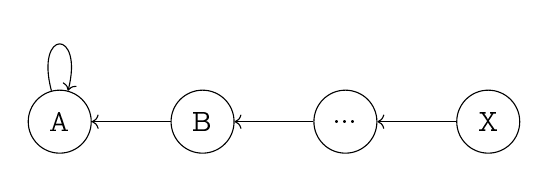
\begin{tikzpicture}[every node/.style={circle, draw, minimum size=8mm},
                  every loop/.style={looseness=10, min distance=5mm}]
    \node (A) {A};
    \node (B)[right=of A] {B};
    \node (C)[right=of B] {...};
    \node (D)[right=of C] {X};
    \draw[->] (A) edge[loop above] (A);
    \draw[->] (B) -- (A);
    \draw[->] (C) -- (B);
    \draw[->] (D) -- (C);
  \end{tikzpicture}
\end{frame}

\begin{frame}[fragile]{\stitle{\subsubsecname -- 路徑壓縮}}
  那麼我們就對於整個要走的路徑去做優化好了!
  \pause

  當我們今天詢問點 $X$ 的時候,我們會希望它與它的結束點的距離 \textbf{越近越好}
  \pause

  而我們在鍊上跑的時候,經過的點好像不是那麼的重要?
  \pause

  所以當我們在詢問完結束點後,是否可以把鍊上經過的所有點的邊,直接連到結束點上?

  \begin{tikzpicture}[every node/.style={circle, draw, minimum size=8mm},
                  every loop/.style={looseness=10, min distance=5mm}]
    \node (A) {A};
    \node (B)[right=of A] {B};
    \node (C)[right=of B] {C};
    \node (D)[right=of C] {D};
    \node (E)[right=of D] {E};
    \draw[->] (A) edge[loop above] (A);
    \draw[->] (B) -- (A);
    \only<4>{
      \draw[->] (C) -- (B);
      \draw[->] (D) -- (C);
      \draw[->] (E) -- (D);
    }
    \only<5>{
      \draw[->,dashed,red] (C) -- (B);
      \draw[->,dashed,red] (D) -- (C);
      \draw[->,dashed,red] (E) -- (D);
      \draw[->,blue] (C) to[out=120,in=30] (A);
      \draw[->,blue] (D) to[out=120,in=40] (A);
      \draw[->,blue] (E) to[out=120,in=50] (A);
    }
  \end{tikzpicture}
\end{frame}

\begin{frame}[fragile]{\stitle{\subsubsecname -- 路徑壓縮}}
  蛤? 這樣還不是要走整條鏈?
  \pause

  這個是 $O((N+Q) \log N)$ 算法?\pause 唬爛吧?
  \pause

  別急,你先別急
  \pause

  我們可以先感性理解一下
  \pause

  當我們每次查詢的時候,都會走完一個鍊的長度,但我們相信他,所以他的長鍊的數量應該只有 $\log N$ 個,所以整體複雜度為 $O((N+Q) \log N)$
  \pause
  ?\pause

  會在之後的章節稍微證明一下正確的複雜度
\end{frame}

\begin{frame}[fragile]{\stitle{\subsubsecname -- 路徑壓縮}}
  路徑壓縮的實作

\begin{lstlisting}
int end_point(int x) {
  if(nxt[x] == x) return x; // 自己是結束點
  // 當前的結束點是下一個點的結束點
  // 直接將下一個點接到查詢後的結束點
  nxt[x] = end_point(nxt[x]); 
  return nxt[x];
}
\end{lstlisting}
\end{frame}

\begin{frame}[fragile]{\stitle{\subsubsecname -- 啟發式合併}}
  啟發式合併 (Union By Rank/Size)
  \pause

  剛剛聊的路徑壓縮是對於詢問結束點的操作所進行的優化
  \pause

  那我們是否可以對合併的時候進行優化呢?
\end{frame}

\begin{frame}[fragile]{\stitle{\subsubsecname -- 啟發式合併}}
  我們發現,當我們做合併連通塊的時候,我們好像是隨便將一個連通塊的結束點連接到另一個連通塊的結束點上
  \pause

  我們可以發現,連接過去的連通塊的最大深度會 $+1$
  \pause

  且換個角度思考,他新接的那條邊最糟會被走下面那個連通塊的節點個數的次數
  \pause

  那麼我們究竟要考慮深度還是節點個數呢?
\end{frame}

\begin{frame}[fragile]{\stitle{\subsubsecname -- 啟發式合併}}
  不難發現,兩種性質都可以影響到之後的複雜度
  \pause

  且兩個連通塊的兩種性質大小關係不一定完全小/大於
  \pause

  所以我們無論選哪個性質來做,複雜度都將會是 $O(\log N)$
  \pause

  複雜度我們以後也會證明
\end{frame}

\begin{frame}[fragile,shrink]{\stitle{\subsubsecname -- 啟發式合併}}
  啟發式合併有兩種做法,而我們這裡使用節點個數總合為啟發式合併的依據

\begin{lstlisting}
// sz[x] 代表著 x 連通塊的大小,預設每個都為 1
void merge(int A, int B) {
  int A_end_point = end_point(A);
  int B_end_point = end_point(B);
  // 相同連通塊不需要合併
  if(A_end_point == B_end_point) return;
  if(sz[A_end_point] > sz[B_end_point]) {
    // 需要將 A 連到 B
    // 且確保 A 的大小 < B 的大小
    swap(A_end_point, B_end_point);
  }
  // 將 A 的結束點連到 B的結束點
  nxt[A_end_point] = B_end_point;
}
\end{lstlisting}
\end{frame}

\subsubsection{複雜度分析}

% \begin{frame}[fragile]{\stitle{\subsubsecname -- 路徑壓縮的複雜度證明}}
  
% \end{frame}

% \begin{frame}[fragile]{\stitle{\subsubsecname -- 啟發式合併的複雜度證明}}
  
% \end{frame}

% \begin{frame}[fragile]{\stitle{\subsubsecname -- 二者皆用的複雜度證明}}
  
% \end{frame}

\begin{frame}[fragile]{\stitle{\subsubsecname -- 總結}}
  有時候路徑壓縮以及啟發式合併並不能套用到某些 DSU 的題目上,但二者只要選一者使用,就能達到 $O(\log N)$ 等級的複雜度
  \pause

  \sout{且理論上複雜度不會證也沒關係}
\end{frame}

\subsubsection{題目}

\begin{frame}[fragile]{\stitle{\subsubsecname -- 例題 1}}
  \begin{problem}
    TOJ 701 電學大師

    $N$ 點,$Q$ 筆詢問

    每次有 $2$ 種操作
    \begin{enumerate}
      \item 連通兩點
      \item 詢問兩點是否有連通
    \end{enumerate}

    題目限制
    \begin{itemize}
      \item $1 \le N \le 10^5$
      \item $1 \le Q \le 2 \times 10^5$
    \end{itemize}
  \end{problem}
\end{frame}

\begin{frame}[fragile]{\stitle{\subsubsecname -- 例題 1}}
  我們可以發現這題是一題 DSU 裸題
  \pause

  而實作上我們通常都是直接寫一個 struct 去把 DSU 的整體架構包住
  \pause

  這樣我們只要確保 struct 裡面的function 寫好,那麼就不會汙染到全域環境了\sout{(也不會佔到變數名稱)}
\end{frame}

\begin{frame}[fragile,shrink]{\stitle{\subsubsecname -- 例題 1}}
  這個是我常用的模板,將連通塊大小跟下一個點的指向寫在一起 \sout{(優美的 code)}

\begin{lstlisting}
struct DSU{
  vector<int> p;
  DSU(int n) : p(n+1, -1) {}
  int fp(int id) {return p[id] < 0 ? id : p[id] = fp(p[id]);}
  bool same(int a, int b) {return fp(a) == fp(b);}
  void upd(int a, int b) {
    int ar = fp(a), br = fp(b);
    if(ar != br) {
      if(p[ar] > p[br]) swap(ar, br);
      p[ar] += p[br];
      p[br] = ar;
    }
  }
};
\end{lstlisting}
\end{frame}

\begin{frame}[fragile,shrink]{\stitle{\subsubsecname -- 例題 1}}
  呼叫

\begin{lstlisting}
// main 裡面
int n, q; cin >> n >> q;
DSU dsu(n);
while(q--) {
  int op, a, b; cin >> op >> a >> b;
  if(op == 0) {
    cout << (dsu.same(a, b) ? "YES\n" : "NO\n");
  } else {
    dsu.upd(a, b);
  }
}
\end{lstlisting}
\end{frame}

\begin{frame}[fragile]{\stitle{\subsubsecname -- 例題 2}}
  \begin{problem}
    TOJ 89 可愛的小動物

    $N$ 個動物,$Q$ 筆詢問

    每次有 $4$ 種操作
    \begin{enumerate}
      \item $A$ 與 $B$ 為朋友
      \item $A$ 與 $B$ 為敵人
      \item 詢問 $A$ 與 $B$ 為朋友
      \item 詢問 $A$ 與 $B$ 為敵人
    \end{enumerate}

    若 $1, 2$ 操作已與之前的操作衝突,則輸出 "angry"

    若 $3, 4$ 操作為真,則輸出 "yeap",反之輸出 "nope"

    題目限制
    \begin{itemize}
      \item $1 \le N, Q \le 5 \cdot 10^5$
    \end{itemize}
  \end{problem}
\end{frame}

\subsection{在線與離線 (Online or Offline)}

\subsection{根號想法 (Sqrt Decomposition)}

\subsection{線段樹 (Segment Tree)}

\subsubsection{單點修改}

\subsubsection{區間修改}

\subsection{樹狀樹組 (Binary Index Tree)}

\subsubsection{單點修改}

\subsubsection{區間修改}

\subsection{稀疏表}

\subsection{珂朵莉樹}

\section{進階資料結構}

\subsection{回滾 DSU}

\subsection{帶權 DSU}

\subsection{線段樹/樹狀數組 上二分搜}

\subsection{字典樹 (Trie)}

\subsection{動態開點線段樹}

\subsection{持久化線段樹}

\subsection{樹套樹}

\subsection{樹堆 (Treap)}

\section{超進階資料結構}

\subsection{李超線段樹}

\subsection{時間線段樹}

\subsection{線段樹優化建圖}

\subsection{吉如一線段樹 (Segment Beat)}

\subsection{持久化 DSU}

\subsection{動態凸包}

\subsection{貓樹}

\section{參考資料}

\begin{frame}[fragile]{\secname}
  \href{https://hackmd.io/quI9kjpkSXGpmzt0XzxeUg}{Tfcis - 2024 寒訓 資料結構簡報 by tobiichi3227}

  \href{https://hackmd.io/@tw20000807/datastructure}{Tfcis T26 資料結構簡報 by tw20000807}

  \href{https://slides.com/tw20000807/deck}{Tfcis - 2024 暑訓 資料結構簡報 by tw20000807}

  \href{https://en.wikipedia.org/wiki/Graph_theory}{Graph\_Theory wiki}

  \href{https://www.researchgate.net/publication/220430653_Worst-case_Analysis_of_Set_Union_Algorithms}{Tarjan, Robert E., van Leeuwen, Jan - Worst-case analysis of set union algorithms}
\end{frame}

\end{document}